% !TeX root = ../report.tex

\section{User Testing}
\subsection{Method}
%General method (what is UT)
%Copy and past of definition
\subsection{Design of the study}
    \subsubsection{User profile and recruitment}
    % Explain the two different user profiles
    \subsubsection{Metrics and indicators}
    % Quantitative and qualitative indicators
    % Scoring
    \subsubsection{Tasks}
    % Tasks list
    % Explain that for each different user profile different task
    We have defined 6 tasks per user profile, so as to further analyze the most relevant sections of the site that we had already inspected in the inspection phase.\\
    Although the tasks assigned to each user profile have been defined according to the importance for the specific user, some tasks overlap because they are interesting for both user profiles.\\
    The site has both simple and complex features so we have defined both simple and complex tasks, so as to simulate the experience of a real user.\\
    \\
    For the user profile “college students that live in Milan” we defined the following tasks:\\
    1. You are a design student at polimi. You want to see what are the major art events of the year, in particular look for the triennale.\\
    2. You are considering which university to enroll to. Try to find out which are the universities in Milan that offer a bachelor degree in economics as an Exchange/International Student.\\
    3. You are an exchange student from US, and you will rent a house here at Milan. Find the required documents to sign a tenancy contract.\\
    4. You want to move around and orient yourself in Milan. Find information and download the map about public transports.\\
    5. You are interested in visiting Milano, but you are unsure of the covid situation of the city and its policies (e.g. regarding green pass). Find more about it and where to get tested.\\
    6. You want to find the list of museums in Milano whose entrance is free. Select the first and look for its opening times, how to reach it and if there are any parking spots.\\
    \\
    For the user profile “tourists that wants to visit the city” we defined the following tasks:\\
    1. For this saturday, you've planned to shop at Porta Venezia till lunch time. Find and book the nearest restaurant in the area for that saturday, in particular you are a vegan.\\
    2. You are planning to book an hotel near the city center (Duomo) for the weekend for two adults, a child and your lovely dog.\\
    3. You are a tourist with three free days, search a suitable itinerary in Milan that may last from one up to three days.\\
    4. You want to move around and orient yourself in Milan. Find information and download the map about public transports.\\
    5. You are interested in visiting Milano, but you are unsure of the covid situation of the city and its policies (e.g. regarding green pass). Find more about it and where to get tested.\\
    6. You want to find the list of museums in Milano whose entrance is free. Select the first and look for its opening times, how to reach it and if there are any parking spots.\\
    
\subsection{Execution of the study}
    % Explain that each inspector had 5 users, 3 students and 2 tourists (or viceversa)
    % Timer, in presence and in remote interview
    % Google form, can include some screenshots
    (unire tale parte con "Design of the study"???)\\
    As stated above, each inspector has recruited 5 users. In particular, two of us have recruited 3 students and 2 tourists and the other two have recruited 2 students and 3 tourists. So we have a total of 20 users, including 10 students and 10 tourists.\\
    To easily collect the data we used a Google Form, the results of which were automatically uploaded to an Excel file. This greatly simplified the process of analysing the results.

\subsection{Results}
    % Final scores (with comments);
    % Aggregates scores (with visualizations)

    We distinguish each user through an ID composed of the type of the profile, the evaluator name and a numerical value, for example Student-1-Alessio identifies the very first student interviewed by Alessio.
\subsubsection{Effectiveness}
    % Effectiveness
    %   - table
    \begin{tabularx}{\linewidth}{l|c|c|c|c|c|c|c|c|c}
    \toprule
    \textbf{User ID} & \textbf{S1} & \textbf{S2} & \textbf{S3} & \textbf{T1} & \textbf{T2} & \textbf{T3} & \textbf{S4-T4} & \textbf{S5-T5} & \textbf{S6-T6} \\
    \midrule
    \endfirsthead
    \toprule
    \textbf{User ID} & \textbf{S1} & \textbf{S2} & \textbf{S3} & \textbf{T1} & \textbf{T2} & \textbf{T3} & \textbf{S4-T4} & \textbf{S5-T5} & \textbf{S5-T5} \\
    \midrule
    \endhead
    \midrule
    \footnotesize [Continues on next page]
    \endfoot
    \bottomrule
    \endlastfoot
        % body
        Alessio-1 & 1 & 1 & 1 &  &  &  & 1 & 1 & 0.5 \\ \midrule
        Alessio-2 & 1 & 1 & 1 &  &  &  & 1 & 1 & 0 \\ \midrule
        Alessio-3 & 0.5 & 1 & 1 &  &  &  & 1 & 1 & 0.5 \\ \midrule
        Andrea-1 & 0.5 & 0.5 & 1 &  &  &  & 1 & 1 & 0.5 \\ \midrule
        Andrea-3 & 1 & 1 & 1 &  &  &  & 1 & 1 & 0 \\ \midrule
        Andrea-5 & 1 & 1 & 1 &  &  &  & 0.5 & 1 & 0.5 \\ \midrule
        Carlo-2 & 0.5 & 1 & 1 &  &  &  & 1 & 1 & 0 \\ \midrule
        Carlo-4 & 1 & 1 & 0 &  &  &  & 1 & 1 & 1 \\ \midrule
        Fabio-1 & 0 & 1 & 0.5 &  &  &  & 1 & 1 & 0 \\ \midrule
        Fabio-2 & 1 & 1 & 1 &  &  &  & 1 & 1 & 0 \\ \midrule
        Alessio-4 &  &  &  & 0 & 1 & 0.5 & 1 & 1 & 1 \\ \midrule
        Alessio-5 &  &  &  & 1 & 1 & 1 & 1 & 1 & 0 \\ \midrule
        Andrea-2 &  &  &  & 1 & 1 & 0 & 1 & 1 & 1 \\ \midrule
        Andrea-4 &  &  &  & 0.5 & 0.5 & 1 & 1 & 1 & 0.5 \\ \midrule
        Carlo-1 &  &  &  & 1 & 1 & 1 & 1 & 1 & 0.5 \\ \midrule
        Carlo-3 &  &  &  & 1 & 0.5 & 1 & 1 & 1 & 0.5 \\ \midrule
        Carlo-5 &  &  &  & 1 & 1 & 1 & 1 & 1 & 1 \\ \midrule
        Fabio-3 &  &  &  & 1 & 1 & 1 & 1 & 1 & 0.5 \\ \midrule
        Fabio-4 &  &  &  & 0.5 & 1 & 1 & 1 & 1 & 0.5 \\ \midrule
        Fabio-5 &  &  &  & 1 & 1 & 1 & 1 & 1 & 0 \\ \midrule
        \textbf{Completion Rate} & \textbf{75\%} & \textbf{95\%} & \textbf{85\%} & \textbf{80\%} & \textbf{90\%} & \textbf{85\%} & \textbf{97\%} & \textbf{100\%} & \textbf{42\%}
    \end{tabularx}

\subsubsection{Efficiency}
    % Efficiency
    %   - table
    %   - Bar chart with (tasks, avg of completion time) for each dataset
    \begin{tabularx}{\linewidth}{l|c|c|c|c|c|c|c|c|c}
    \toprule
    \textbf{User ID} & \textbf{S1} & \textbf{S2} & \textbf{S3} & \textbf{T1} & \textbf{T2} & \textbf{T3} & \textbf{S4-T4} & \textbf{S5-T5} & \textbf{S6-T6} \\
    \midrule
    \endfirsthead
    \toprule
    \textbf{User ID} & \textbf{S1} & \textbf{S2} & \textbf{S3} & \textbf{T1} & \textbf{T2} & \textbf{T3} & \textbf{S4-T4} & \textbf{S5-T5} & \textbf{S5-T5} \\
    \midrule
    \endhead
    \midrule
    \footnotesize [Continues on next page]
    \endfoot
    \bottomrule
    \endlastfoot
        % body
        Alessio-1 & 2:23 & 0:52 & 2:12 &  &  &  & 3:25 & 0:49 & 9:47 \\ \midrule
        Alessio-2 & 1:26 & 1:13 & 2:04 &  &  &  & 1:35 & 1:45 & 7:55 \\ \midrule
        Alessio-3 & 4:04 & 0:57 & 2:01 &  &  &  & 4:19 & 1:18 & 6:43 \\ \midrule
        Andrea-1 & 0:54 & 2:35 & 1:05 &  &  &  & 0:45 & 0:08 & 2:43 \\ \midrule
        Andrea-3 & 1:36 & 2:05 & 0:56 &  &  &  & 0:55 & 0:15 & 1:43 \\ \midrule
        Andrea-5 & 0:34 & 0:53 & 1:10 &  &  &  & 1:20 & 0:10 & 2:24 \\ \midrule
        Carlo-2 & 4:54 & 1:36 & 3:16 &  &  &  & 0:35 & 0:40 & 5:35 \\ \midrule
        Carlo-4 & 3:23 & 1:12 & 4:48 &  &  &  & 1:16 & 1:10 & 3:59 \\ \midrule
        Fabio-1 & 8:00 & 2:37 & 2:30 &  &  &  & 3:20 & 0:33 & 9:09 \\ \midrule
        Fabio-2 & 4:25 & 1:25 & 1:55 &  &  &  & 0:49 & 0:30 & 1:40 \\ \midrule
        Alessio-4 &  &  &  & 14:30 & 6:10 & 5:05 & 2:51 & 1:00 & 8:13 \\ \midrule
        Alessio-5 &  &  &  & 1:12 & 1:40 & 0:35 & 2:05 & 0:35 & 11:16 \\ \midrule
        Andrea-2 &  &  &  & 0:57 & 0:47 & 1:17 & 0:34 & 0:07 & 1:57 \\ \midrule
        Andrea-4 &  &  &  & 0:56 & 1:54 & 0:44 & 0:31 & 0:20 & 3:54 \\ \midrule
        Carlo-1 &  &  &  & 1:46 & 1:52 & 0:53 & 0:46 & 1:14 & 3:51 \\ \midrule
        Carlo-3 &  &  &  & 0:50 & 1:50 & 0:50 & 0:58 & 1:36 & 3:05 \\ \midrule
        Carlo-5 &  &  &  & 1:56 & 2:20 & 2:55 & 1:24 & 0:20 & 2:30 \\ \midrule
        Fabio-3 &  &  &  & 2:16 & 1:07 & 0:30 & 0:34 & 0:23 & 5:33 \\ \midrule
        Fabio-4 &  &  &  & 5:00 & 2:12 & 0:50 & 4:35 & 0:20 & 7:20 \\ \midrule
        Fabio-5 &  &  &  & 4:33 & 1:42 & 0:58 & 1:17 & 0:45 & 9:12 \\ \midrule
        \textbf{Average Time} & \textbf{3:09} & \textbf{1:32} & \textbf{2:11} & \textbf{3:23} & \textbf{2:09} & \textbf{1:27} & \textbf{1:49} & \textbf{0:43} & \textbf{5:09}
    \end{tabularx}

\subsubsection{Errors}
    % Errors
    %   - Bar chart with (tasks, avg of errors) for each dataset
    \begin{figure}[!ht]
        \begin{minipage}{\linewidth}
            \centering
            \makebox[\textwidth][c]{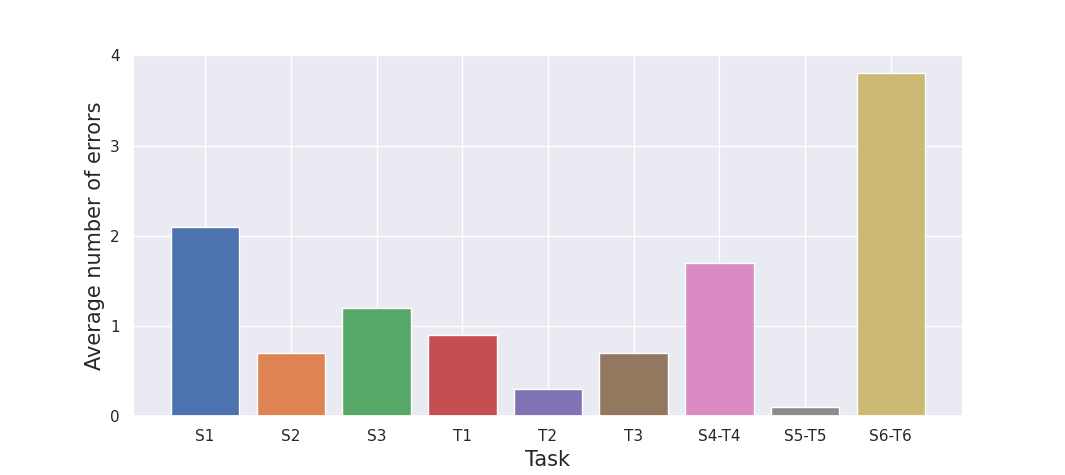
\includegraphics[width=1.2\textwidth]{images/BarsErrors.png}}%
            \captionsetup{justification=centering}
            \caption{Average of user errors for each task}
            \label{BarsErrors}
        \end{minipage}
    \end{figure}

\subsubsection{Task difficulty}
    % Task difficulty
    %   - Linee spezzate per ogni task, con una linea spessa per avg (tester, voto)


\subsection{Discussion of results}
    % Your observations on results
    % Summary of comments from user testing